\documentclass{beamer}

\usepackage[utf8x]{inputenc}
\usepackage{graphicx}
\usepackage{amsthm,amssymb,amsbsy,amsmath,amsfonts,amssymb,amscd}
\usepackage{dsfont}
\usepackage{array}
\usepackage{tikz}
\newcolumntype{N}{@{}m{2pt}@{}}
\useoutertheme[subsection=false]{miniframes}
\usepackage{lmodern}

%%%%%%%%%%%%%%%%%%%%%%%%
% GENERAL BEAMER STYLE :

\setbeamertemplate{footline}{
  \hbox{%
    \begin{beamercolorbox}[wd=.2\paperwidth,ht=2ex,dp=1ex,left]{author in head/foot}%
      \hskip1em\usebeamerfont{author in head/foot}\insertshortauthor
    \end{beamercolorbox}%
    \begin{beamercolorbox}[wd=.7\paperwidth,ht=2ex,dp=1ex,center]{title in head/foot}%
      \usebeamerfont{title in head/foot}\insertshorttitle
    \end{beamercolorbox}%
    \begin{beamercolorbox}[wd=.1\paperwidth,ht=2ex,dp=1ex,right]{page number in head/foot}%
      \usebeamerfont{page number in head/foot}\insertframenumber{} / \inserttotalframenumber
      \kern1em 
    \end{beamercolorbox}
  }
}

\setbeamercolor{alerted text}{fg=red!80!black}
\setbeamercolor{itemize/enumerate subbody}{fg=gray!70!black}
\setbeamertemplate{itemize item}[square]
\setbeamertemplate{itemize subitem}[triangle]%{{\textendash}}
\setbeamerfont{itemize/enumerate subbody}{size=\footnotesize}
\setbeamerfont{itemize/enumerate subitem}{size=\footnotesize}

\setbeamertemplate{navigation symbols}{}

\AtBeginSection{
\begin{frame}
    \begin{centering}
    \begin{beamercolorbox}[sep=12pt,center]{part title}
    \usebeamerfont{section title}\insertsection\par
    \end{beamercolorbox}
    \end{centering}
\end{frame}
}

 



\title[Short course on Statistical Modeling for Optimization -- lecture 4/4]{ \small Short course on Statistical Modelling for Optimization -- lecture 4/4 \\ \vspace{3mm} \LARGE Global optimization with GPs}
\institute[Mines St-\'Etienne]{Nicolas Durrande (durrande@emse.fr) \\ Jean-Charles Croix (jean-charles.croix@emse.fr) \\ Mines St-\'Etienne -- France}
\author[Pereira, June 2016]{June 2016 -- Universidad Tecnol\'ogica de Pereira -- Colombia}
\date{\null}

\DeclareMathOperator*{\Var}{var}
\DeclareMathOperator*{\E}{E}
\DeclareMathOperator*{\Cov}{cov}
\newcommand\PR[1]{\mathrm{P}\left(#1 \right)}
\newcommand\PS[1]{{\langle #1 \rangle}_\mathcal{H}}
\newcommand\PSi[2]{{ \left \langle #1 \right \rangle}_{\! #2}}
\newcommand\N[1]{{|| #1 ||}_\mathcal{H}}
\newcommand\Ni[2]{{|| #1 ||}_{\! #2}}
\newcommand\dx{\, \mathrm{d}}
\newcommand\textequal{\rule[.4ex]{4pt}{0.4pt}\llap{\rule[.7ex]{4pt}{0.4pt}}}
\newcommand{\argmin}{\operatornamewithlimits{argmin}}
\makeatletter
\newcommand{\shorteq}{%
  \settowidth{\@tempdima}{a}% Width of hyphen
  \resizebox{\@tempdima}{\height}{=}%
}
\makeatother

\definecolor{Orange}{rgb}{0.8,0.1470,0.0}
\definecolor{MonBleu}{rgb}{0.212, 0.392, 0.545}
%%%%%%%%%%%%%%%%%%%%%%%%%%%%%%%%%%%%%%%%%%%%%%%%%%%%%%
%%%%%%%%%%%%%%%%%%%%%%%%%%%%%%%%%%%%%%%%%%%%%%%%%%%%%%
%%%%%%%%%%%%%%%%%%%%%%%%%%%%%%%%%%%%%%%%%%%%%%%%%%%%%%
\begin{document}
\setbeamercolor{author in head/foot}{fg=gray,bg=white}
\setbeamercolor{title in head/foot}{fg=gray,bg=white}
\setbeamercolor{page number in head/foot}{fg=gray,bg=white}
\setbeamercolor{section in head/foot}{bg=black,fg=gray}
\setbeamercolor{subsection in head/foot}{bg=black,fg=gray}

%%%%%%%%%%%%%%%%%%%%%%%%%%%%%%%%%%%%%%%%%%%%%%%%%%%%%%
\begin{frame}
  \titlepage
\end{frame}

%%%%%%%%%%%%%%%%%%%%%%%%%%%%%%%%%%%%%%%%%%%%%%%%%%%%%%
\begin{frame}{}
Today will be the last lecture
\vspace{0.2cm}
\begin{itemize}
	\item Motivations
	\item Usual optimization methods
	\item Efficient Global Optimization
	\item Solving inverse problems
\end{itemize}
\end{frame}

%%%%%%%%%%%%%%%%%%%%%%%%%%%%%%%%%%%%%%%%%%%%%%%%%%%%%%
%%%%%%%%%%%%%%%%%%%%%%%%%%%%%%%%%%%%%%%%%%%%%%%%%%%%%%
\section{Introduction}
\subsection{}

%%%%%%%%%%%%%%%%%%%%%%%%%%%%%%%%%%%%%%%%%%%%%%%%%%%%%%
\begin{frame}{}
Optimization is one of the most common problem in engineering. \\
\vspace{4mm}
One can distinguish methodologies:
\begin{itemize}
	\item Local optimization
	\item Global optimization
	\item Robust optimization
\end{itemize}
and different function input spaces:
\begin{itemize}
	\item Discrete
	\item Continuous
\end{itemize}
\vspace{5mm}
We usually consider as a reference the  \textbf{minimization} problem, and this course is about continuous variables\\
\end{frame}

%%%%%%%%%%%%%%%%%%%%%%%%%%%%%%%%%%%%%%%%%%%%%%%%%%%%%%
\begin{frame}{}
According to the context of this short course, we will focus on optimization methods that do not require a lot of function evaluations.\\
$\rightarrow$ model based optimization.\\
\vspace{5mm}
We will also pay a particular attention to optimization when
	\begin{itemize}
	 	\item observations are noisy
	 	\item parameter values are noisy
	 \end{itemize} 
\end{frame}

%%%%%%%%%%%%%%%%%%%%%%%%%%%%%%%%%%%%%%%%%%%%%%%%%%%%%%
%%%%%%%%%%%%%%%%%%%%%%%%%%%%%%%%%%%%%%%%%%%%%%%%%%%%%%
\section{Local optimization}
\subsection{}

%%%%%%%%%%%%%%%%%%%%%%%%%%%%%%%%%%%%%%%%%%%%%%%%%%%%%%
\begin{frame}{}
Local optimization methods are looking for the minimum value that can be found in the ``neighbourhood'' of the starting point.\\
\vspace{5mm}
Typical method is \textbf{gradient descent}.\\
\vspace{5mm}
\begin{center}
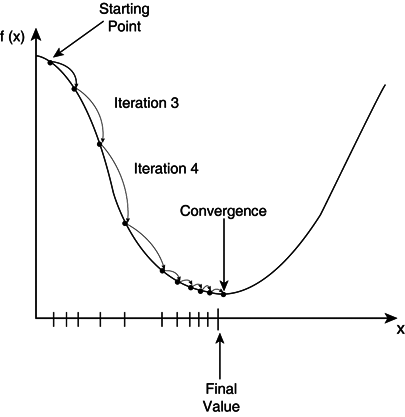
\includegraphics[height=5cm]{figures/grad_desc1}
\end{center}
\end{frame}

%%%%%%%%%%%%%%%%%%%%%%%%%%%%%%%%%%%%%%%%%%%%%%%%%%%%%%
\begin{frame}{}
This can also be done in higher dimension:\\
\vspace{5mm}
\begin{center}
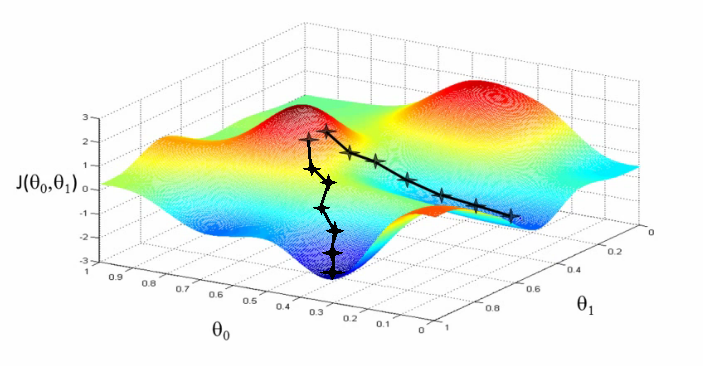
\includegraphics[height=6cm]{figures/grad_desc2}
\end{center}
The convergence points depends on the starting region.
\end{frame}

%%%%%%%%%%%%%%%%%%%%%%%%%%%%%%%%%%%%%%%%%%%%%%%%%%%%%%
\begin{frame}{}
Cons of gradient descent:
\begin{itemize}
	\item cannot handle noise
	\item in high dimension, computing the gradient is costly
 	\item it does not follow the shortest path
 \end{itemize} 
\begin{center}
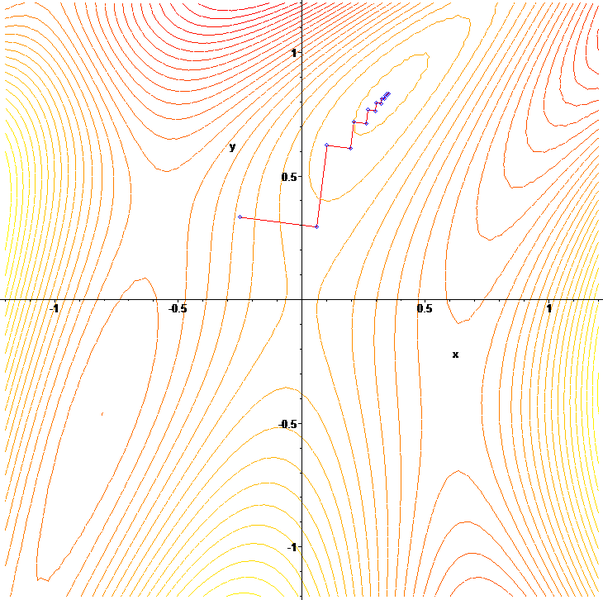
\includegraphics[height=5cm]{figures/grad_desc3}
\end{center}
\begin{center}
The convergence points depends on the starting region.
\end{center}
\end{frame}

%%%%%%%%%%%%%%%%%%%%%%%%%%%%%%%%%%%%%%%%%%%%%%%%%%%%%%
\begin{frame}{}
Observation noise is always an issue for gradient based methods:\\
\vspace{2mm}
\begin{center}
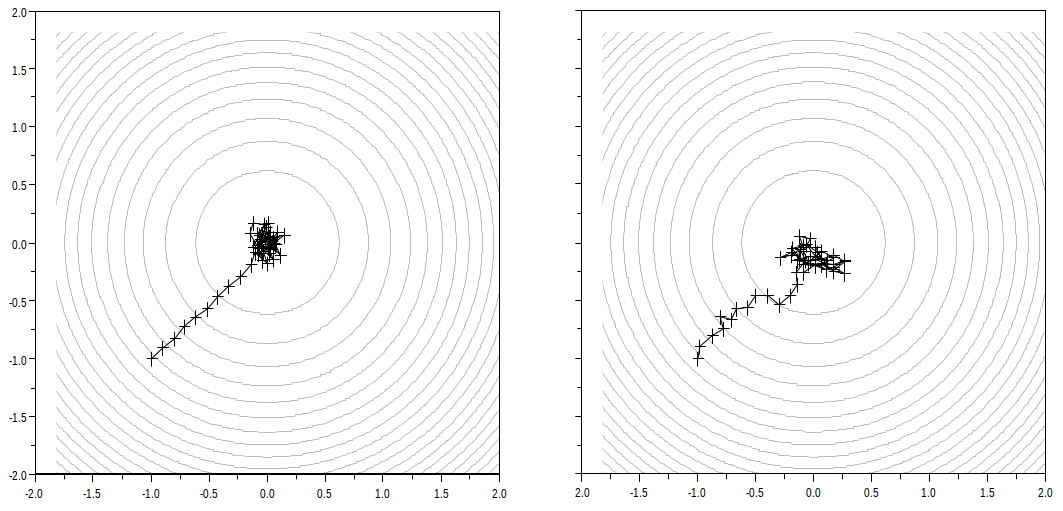
\includegraphics[height=5cm]{figures/RLRgraddesc}\\
Deterministic \hspace{2.8cm} Noisy observations
\end{center}
\small Source: Talk from R. Le Riche at the \emph{Modeling and Numerical Methods for Uncertainty Quantification}, Porquerolles, 2014
\end{frame}

%%%%%%%%%%%%%%%%%%%%%%%%%%%%%%%%%%%%%%%%%%%%%%%%%%%%%%
\begin{frame}{}
One improvement is to consider not only the first derivative but also higher orders\\
\vspace{3mm}
\textbf{Newton methods}
The sequence of visited points is given by:
$$ x_{n+1} = x_n - \frac{f'(x_n)}{f''(x_n)} $$
This can be interpreted as fitting a quadratic function at each step and to define the next point as the maximum/minimum of the quadratic function.
\end{frame}

%%%%%%%%%%%%%%%%%%%%%%%%%%%%%%%%%%%%%%%%%%%%%%%%%%%%%%
\begin{frame}{}
In higher dimension, the first and second derivatives are replaced by the gradient and the Hessian matrix:
$$ x_{n+1} = x_n - (H_f(x_n))^{-1} \nabla f(x_n) $$
\begin{columns}[c]
\column{5cm}
\begin{itemize}
	\item[+] The convergence is faster than gradient descent
	\item[$-$] Does not handle noise
	\item[$-$] Computationally expensive (Hessian matrix)
\end{itemize}
\column{5cm}
\begin{center}
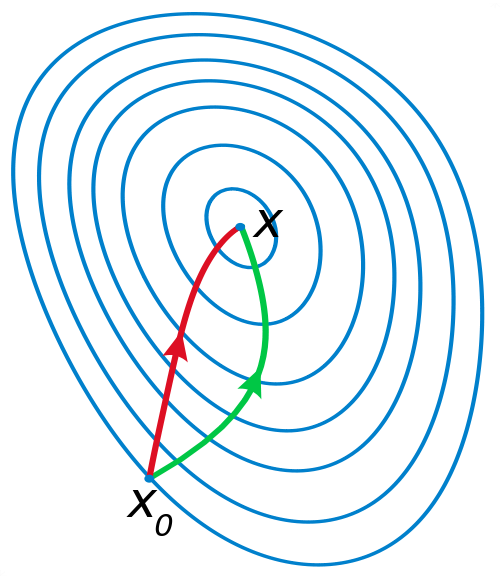
\includegraphics[height=5cm]{figures/newton}
\end{center}
\end{columns}
\end{frame}

%%%%%%%%%%%%%%%%%%%%%%%%%%%%%%%%%%%%%%%%%%%%%%%%%%%%%%
\begin{frame}{}
In order to overcome the expensive computation of the Hessian matrix, \textbf{Quasi Newton methods} use an approximation of it based on low rank updates.\\
\vspace{5mm}
\textbf{BFGS} is probably the most famous example.
\begin{itemize}
	\item[+] They are fast algorithm
	\item[+] Already implemented in all languages
	\item[$-$] Requires a large number of evaluations
	\item[$-$] Cannot handle noise
\end{itemize}
\end{frame}

%%%%%%%%%%%%%%%%%%%%%%%%%%%%%%%%%%%%%%%%%%%%%%%%%%%%%%
\begin{frame}{}
In practice, we are often interested in the \textbf{global minimum} and not just the local ones:
\begin{center}
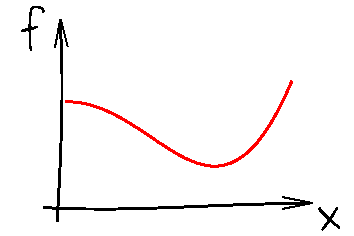
\includegraphics[height=4.5cm]{figures/ink_f}
\end{center}
Cheap improvements are: 
\begin{itemize}
 	\item \textbf{multi-start}.
 	\item Monte-Carlo + BFGS
\end{itemize} 
\end{frame}

%%%%%%%%%%%%%%%%%%%%%%%%%%%%%%%%%%%%%%%%%%%%%%%%%%%%%%
%%%%%%%%%%%%%%%%%%%%%%%%%%%%%%%%%%%%%%%%%%%%%%%%%%%%%%
\section{Global optim.}
\subsection{}

%%%%%%%%%%%%%%%%%%%%%%%%%%%%%%%%%%%%%%%%%%%%%%%%%%%%%%
\begin{frame}{}
A wide variety of global optimization methods have been developed:
\begin{itemize}
	\item Evolutionary algorithms
	\item Simulated annealing
	\item Model based optimization
\end{itemize}
\end{frame}

%%%%%%%%%%%%%%%%%%%%%%%%%%%%%%%%%%%%%%%%%%%%%%%%%%%%%%
\begin{frame}{Evolutionary algorithms}
The principle of \textbf{evolutionary algorithm} is to consider a population of points that will change at each time step. The evolution of the population is typically done by:
\begin{itemize}
	\item selecting the best points (Parents)
	\item combining points together (Breeding)
	\item mutations of points
\end{itemize}
\end{frame}

%%%%%%%%%%%%%%%%%%%%%%%%%%%%%%%%%%%%%%%%%%%%%%%%%%%%%%
\begin{frame}{Evolutionary algorithms}
A state of the art evolutionary algorithm for optimization is \textbf{CMA-ES} (Covariance Matrix Adaptation Evolution Strategy): \\
\vspace{3mm}
Starting from an initial set of normally distributed points, the algorithm loops over
\begin{itemize}
	\item[1.] select the best subset of points
	\item[2.] update the distribution mean
	\item[3.] update the covariance matrix
	\item[4.] generate a new set of points
\end{itemize}
\vspace{5mm}
\structure{Remarks:} no gradient is computed. The algorithm can handle noise.\\
\end{frame}

%%%%%%%%%%%%%%%%%%%%%%%%%%%%%%%%%%%%%%%%%%%%%%%%%%%%%%
\begin{frame}{Example: steps of the CMA-ES algorithm}
\begin{enumerate}
	\item Sampling ($\lambda$ individuals, $g$ generation) and evaluating:
	\[
	x_k^{g+1}=m^g+\sigma^g\mathcal{N}(0,C^g),\;k=1..\lambda\Rightarrow f(x_k^{g+1})
	\]
	\item Selection and recombination:
	\[
	m^{g+1}=\sum_{i=1}^\mu{w_ix_{i:\lambda}^{g+1}},\sum_{i=1}^\mu{w_i}=1,\;w_1\geq...\geq w_\mu\geq 0
	\]
	\item Covariance update (multiple methods...):
	\[
	C_\mu^{g+1}=\sum_{i=1}^\mu{w_i(x_{i:\lambda}^{g+1}-m^g)(x_{i:\lambda}^{g+1}-m^g)^T}
	\]
\end{enumerate}
\small Source: The CMA Evolution Strategy: A Tutorial, N. Hansen, 2016 
\end{frame}

%%%%%%%%%%%%%%%%%%%%%%%%%%%%%%%%%%%%%%%%%%%%%%%%%%%%%%
\begin{frame}{Evolutionary algorithms}
\begin{example}
\begin{center}
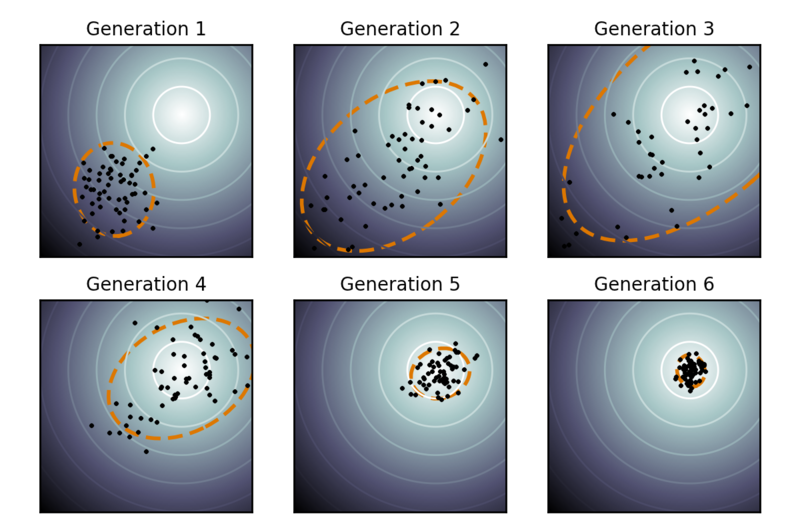
\includegraphics[height=7cm]{figures/CMAES}
\end{center}	
\end{example}
\end{frame}

%%%%%%%%%%%%%%%%%%%%%%%%%%%%%%%%%%%%%%%%%%%%%%%%%%%%%%
\begin{frame}{Simulated annealing}
The principle of simulated annealing is to consider a random walk in the input space and to accept the move from $x_n$ to $x_{n+1}$ if either
\begin{itemize}
	\item $f(x_{n+1}) < f(x_{n})$ (the moves improve the criteria)
	\item $\exp(-(f(x_{n+1})-f(x_{n}))/T) < U$ where U is a uniform(0,1) random variable and $T$ is the temperature (we accept ``small'' degradations).
\end{itemize}
\vspace{3mm}
Simulated annealing is inspired from a metallurgy technique involving heating and controlled cooling of materials to improve the structure.
\vspace{3mm}
Allowing moves that degrade the function allows to escape from local minima.\\
\vspace{3mm}
$T$ must tends toward zero with time to obtain convergence
\end{frame}

%%%%%%%%%%%%%%%%%%%%%%%%%%%%%%%%%%%%%%%%%%%%%%%%%%%%%%
\begin{frame}{Simulated annealing}
\textbf{Pros:}
\begin{itemize}
	\item No need for gradients
	\item Can be used in high dimension
	\item Provides a trade-off exploitation/optimization
\end{itemize}
\vspace{3mm}
\textbf{Cons:}
\begin{itemize}
	\item The temperature is difficult to tune
	\item Requires a large number of observations
\end{itemize}
\end{frame}

%%%%%%%%%%%%%%%%%%%%%%%%%%%%%%%%%%%%%%%%%%%%%%%%%%%%%%
%%%%%%%%%%%%%%%%%%%%%%%%%%%%%%%%%%%%%%%%%%%%%%%%%%%%%%
\section[Model based optim.]{Model based optimization methods}
\subsection{}

%%%%%%%%%%%%%%%%%%%%%%%%%%%%%%%%%%%%%%%%%%%%%%%%%%%%%%
\begin{frame}{}
If the number of function evaluations are limited, we can run the optimization on the model instead of running it directly on the function
\begin{center}
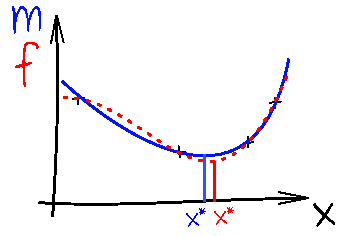
\includegraphics[height=5cm]{figures/ink_mf}
\end{center}
In the end, we hope that:
\begin{equation}
	\begin{split}
		\argmin(m) & \approx \argmin(f)\\
		\min(m) & \approx \min(f)\\
	\end{split}
\end{equation}
\end{frame}

%%%%%%%%%%%%%%%%%%%%%%%%%%%%%%%%%%%%%%%%%%%%%%%%%%%%%%
\begin{frame}{}
\structure{Overall framework}
  \begin{figure}
    \centering \sf
    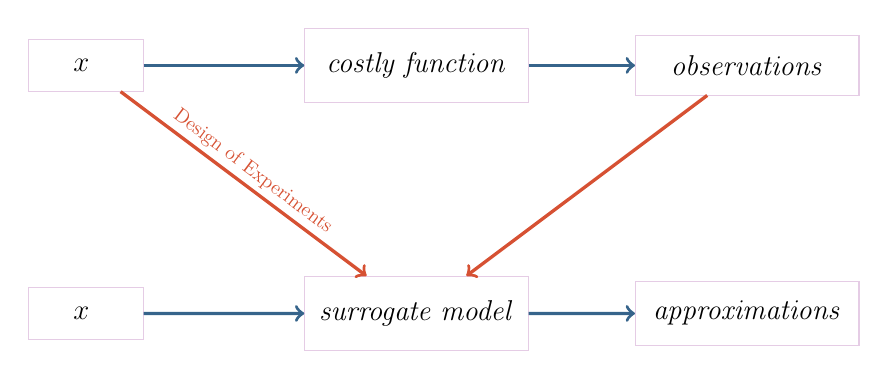
\begin{tikzpicture}[scale=0.7, every node/.style={scale=0.6}]
     
      % \tikzstyle{Sim}=[rectangle, draw=MonBleu!20, fill=MonBleu!0];
      % \tikzstyle{Meta}=[rectangle, draw=Orange!40, fill=MonBleu!0];
      \tikzstyle{Mes}=[rectangle, draw=violet!20, fill=violet!0];

        \node[Mes](MesIn) at (-6, 0) {
          \parbox{2.2cm}{ % 
            \centering
            \LARGE 
            \vspace{3mm}
            $x$
            \vspace{3mm}
          }};

        \node[Mes](Mes) at (0, 0) {
          \parbox{4.5cm}{ % 
            \centering
            \LARGE 
            \vspace{4mm}
            \textit{costly function}\\
            \vspace{4mm}
          }};
        
        \node[Mes](MesOut) at (6, 0) {
        \parbox{4.5cm}{ % 
            \centering
            \LARGE 
            \vspace{3mm}
          \textit{observations}\\
            \vspace{3mm}
        }};
        \draw[->, very thick, draw=MonBleu] (MesIn) -- (Mes.west);
        \draw[->, very thick, draw=MonBleu] (Mes) -- (MesOut.west);
        
        \node[Mes](MetaIn) at (-6, -4.5) {
          \parbox{2.2cm}{ % 
          \centering
            \LARGE 
            \vspace{3mm}
            $x$
            \vspace{3mm}
          }};
        
        \node[Mes](Meta) at (0, -4.5) {
          \parbox{4.5cm}{ % 
            \centering
            \LARGE 
            \vspace{4mm}
            \textit{surrogate model}\\
            \vspace{4mm}
          }};
        
        \node[Mes](MetaOut) at (6.0, -4.5) {
        \parbox{4.5cm}{ % 
            \centering
            \LARGE 
            \vspace{3mm}
          \textit{approximations}\\
            \vspace{3mm}
        }};
        
        \draw[->, very thick, draw=MonBleu] (MetaIn) -- (Meta.west);
        \draw[->, very thick, draw=MonBleu] (Meta) -- (MetaOut.west);
 
        \draw[->, very thick, draw=Orange!80] (MesIn) -- (Meta)
        node [above, midway, sloped, Orange!80] {\large Design of Experiments}; 
        \draw[->, very thick, draw=Orange!80] (MesOut)  -- (Meta);
        %node [above, midway, sloped, Orange!80] {\large réponses}; 

    \end{tikzpicture}
    \end{figure}  
In practice, it is risky to take decisions based only on the model...\\
\vspace{3mm} 
On the other hand, the model can be used to guide us in the search for the optimum. 
\end{frame}

%%%%%%%%%%%%%%%%%%%%%%%%%%%%%%%%%%%%%%%%%%%%%%%%%%%%%%
\begin{frame}{}
Global optimization methods are a trade-off between 
\begin{itemize}
	\item Exploitations of good results
	\item Exploration of the space
\end{itemize}
\vspace{3mm}
\begin{center}
\textbf{How can GPR models be helpful?}\\
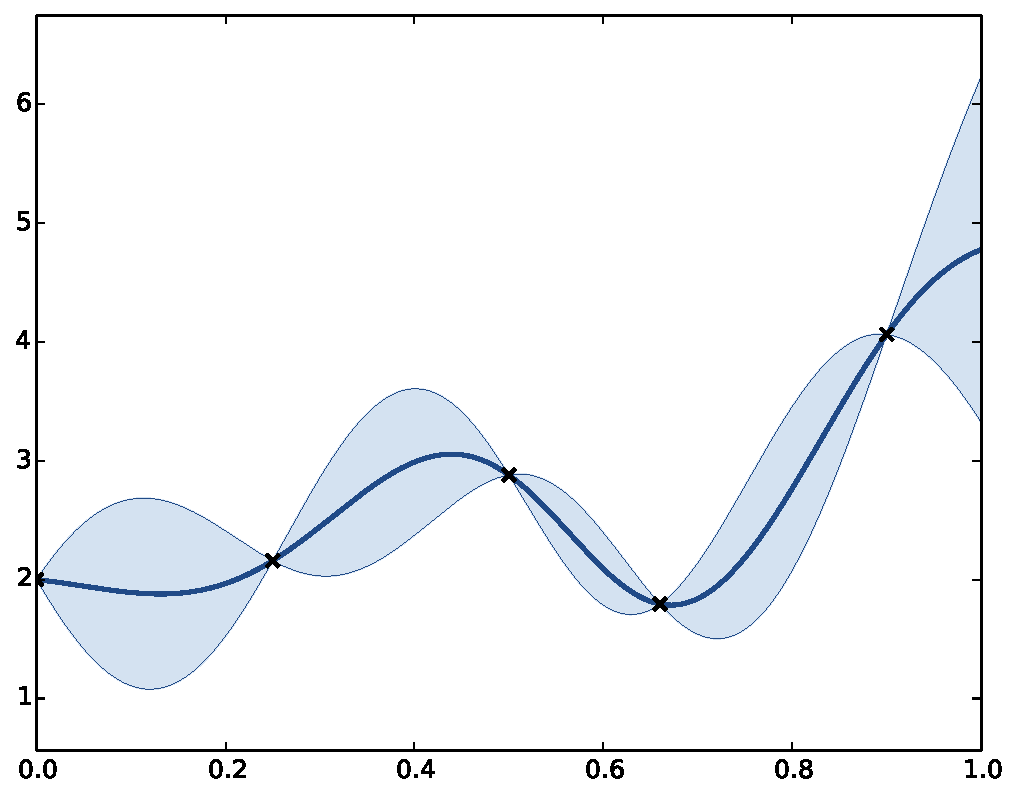
\includegraphics[height=5cm]{figures/python/ego_0}
\end{center}
\end{frame}

%%%%%%%%%%%%%%%%%%%%%%%%%%%%%%%%%%%%%%%%%%%%%%%%%%%%%%
\begin{frame}{}
In our example, the best observed value is 1.79
\begin{center}
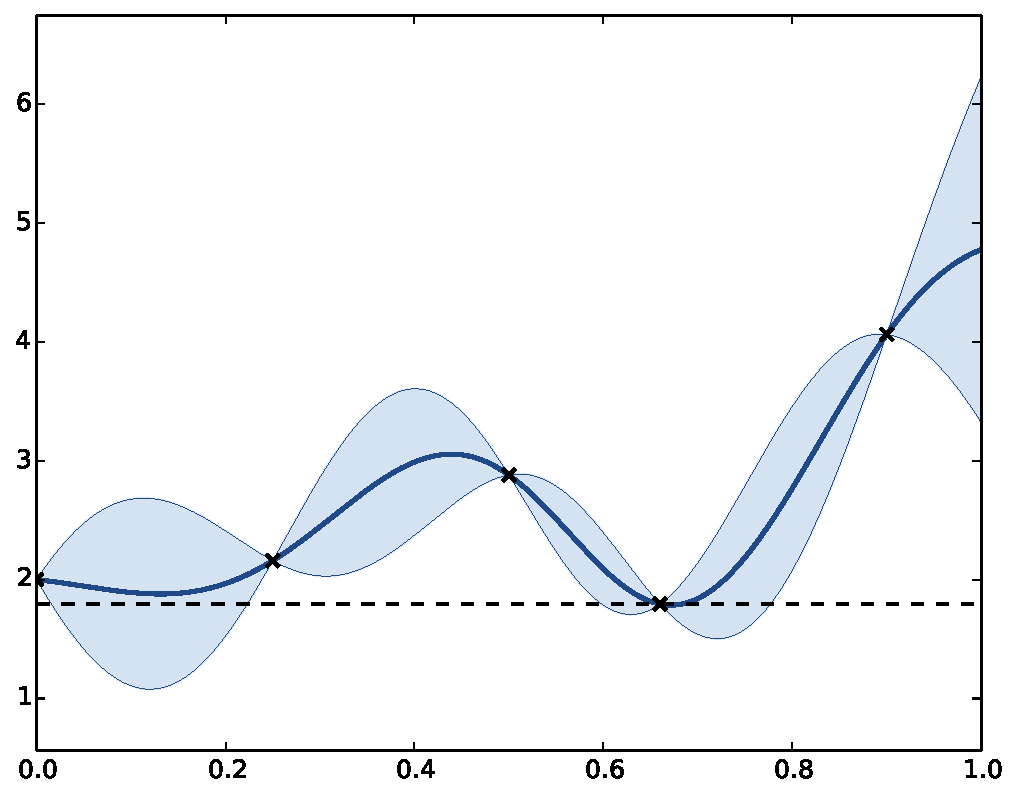
\includegraphics[height=5cm]{figures/python/ego_improv}
\end{center}
Various criteria can be studied
\begin{itemize}
	\item probability of improvement
	\item Expected improvement
\end{itemize}
\end{frame}

%%%%%%%%%%%%%%%%%%%%%%%%%%%%%%%%%%%%%%%%%%%%%%%%%%%%%%
\begin{frame}{}
\textbf{Probability of Improvement:}
$$PI(x) = cdf \left(\frac{\min(F) - m(x)}{\sqrt{(c(x,x))}} \right)$$
\begin{center}
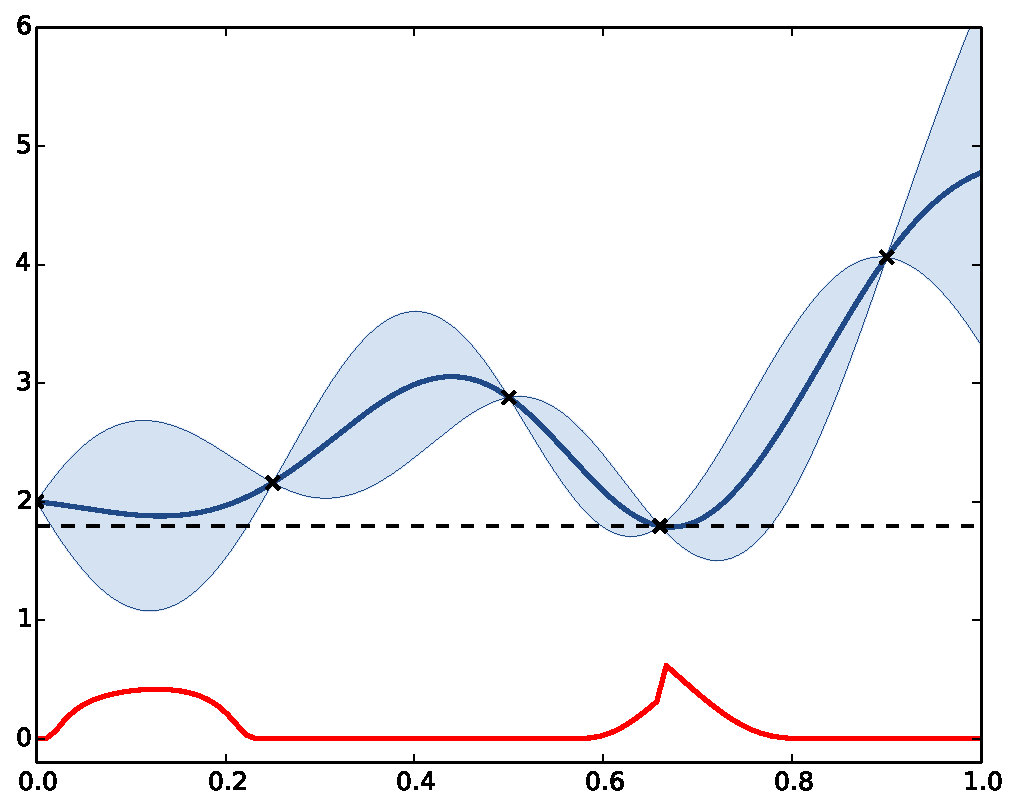
\includegraphics[height=5cm]{figures/python/ego_PI}
\end{center}
\end{frame}

%%%%%%%%%%%%%%%%%%%%%%%%%%%%%%%%%%%%%%%%%%%%%%%%%%%%%%
\begin{frame}{}
The point with the highest PI is often very close to the best observed value. We can show that there is a $x$ in the neighbourhood of $x^*$ such that $PI(x) \geq 0.5$.\\
\vspace{5mm}
For such points, the improvement cannot be large... \\
\vspace{3mm}
Can we find another criterion?
\end{frame}

%%%%%%%%%%%%%%%%%%%%%%%%%%%%%%%%%%%%%%%%%%%%%%%%%%%%%%
\begin{frame}{}
\textbf{Expected Improvement:}
$$EI(x) = \sqrt{c(x,x)} (u(x) cdf(u(x)) + pdf(u(x)))$$
\qquad with $ \displaystyle u(x) = \frac{\min(F) - m(x)}{\sqrt{(c(x,x))}}$
\begin{center}
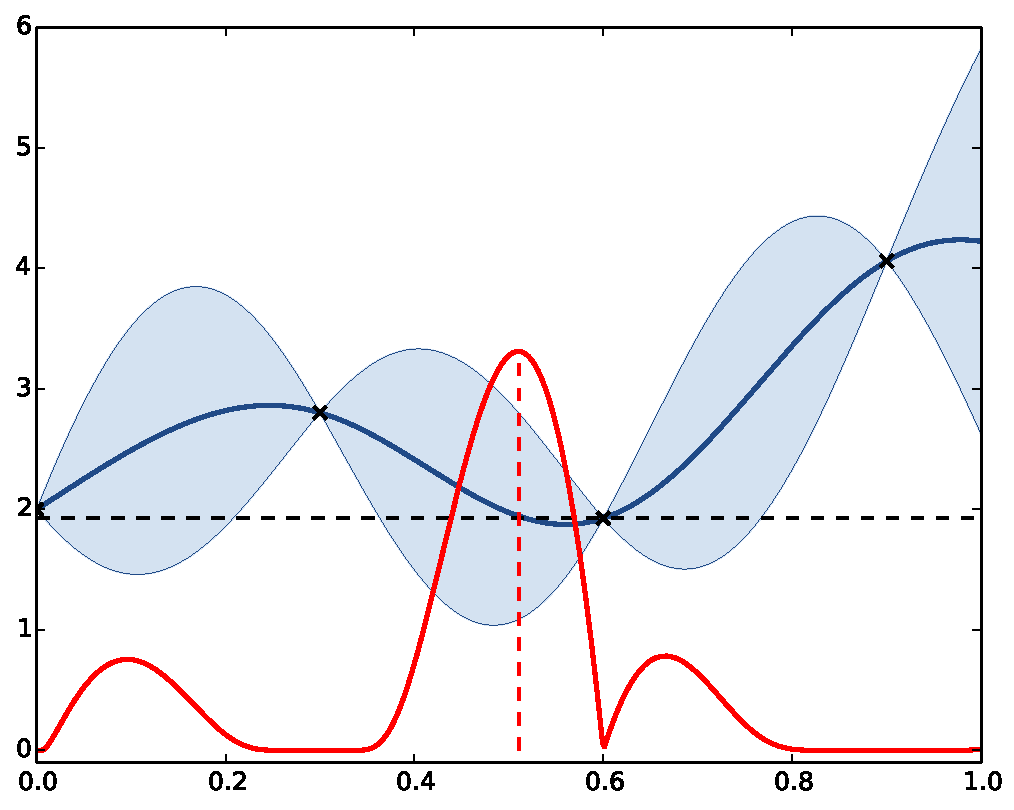
\includegraphics[height=5cm]{figures/python/ego_EI0}
\end{center}
\end{frame}

%%%%%%%%%%%%%%%%%%%%%%%%%%%%%%%%%%%%%%%%%%%%%%%%%%%%%%
\begin{frame}{Expected Improvement}
Let's see how it works... iteration 1
\begin{center}
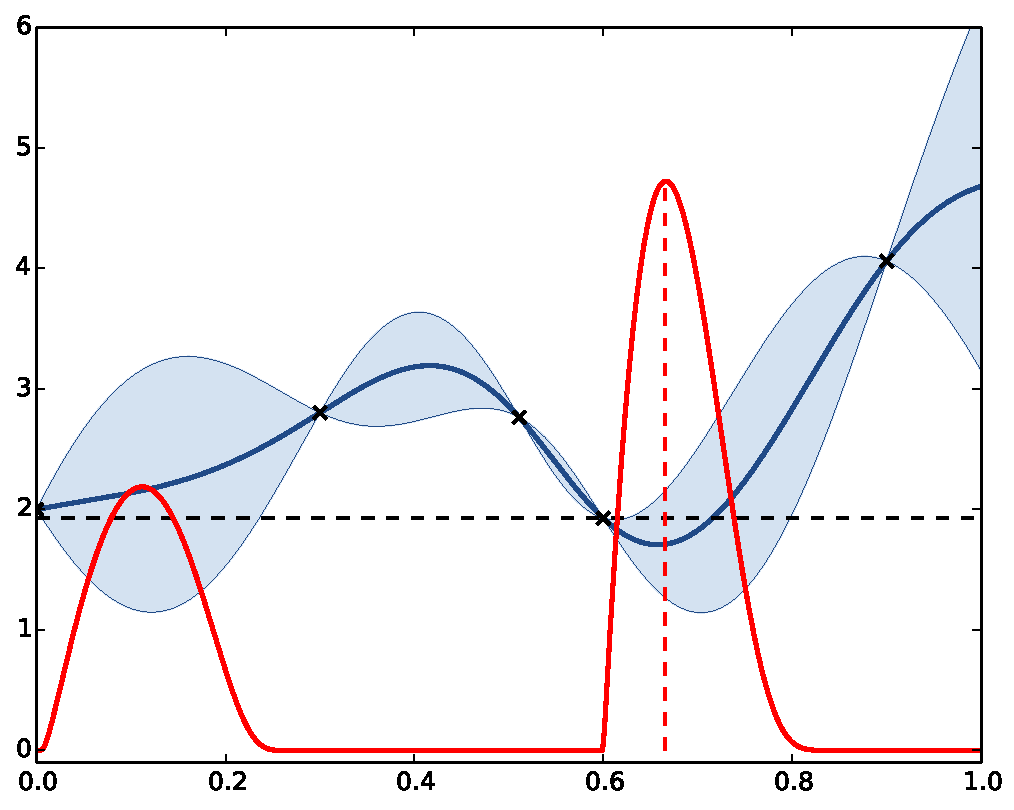
\includegraphics[height=5cm]{figures/python/ego_EI1}
\end{center}
\end{frame}

%%%%%%%%%%%%%%%%%%%%%%%%%%%%%%%%%%%%%%%%%%%%%%%%%%%%%%
\begin{frame}[noframenumbering]{Expected Improvement}
Let's see how it works... iteration 2
\begin{center}
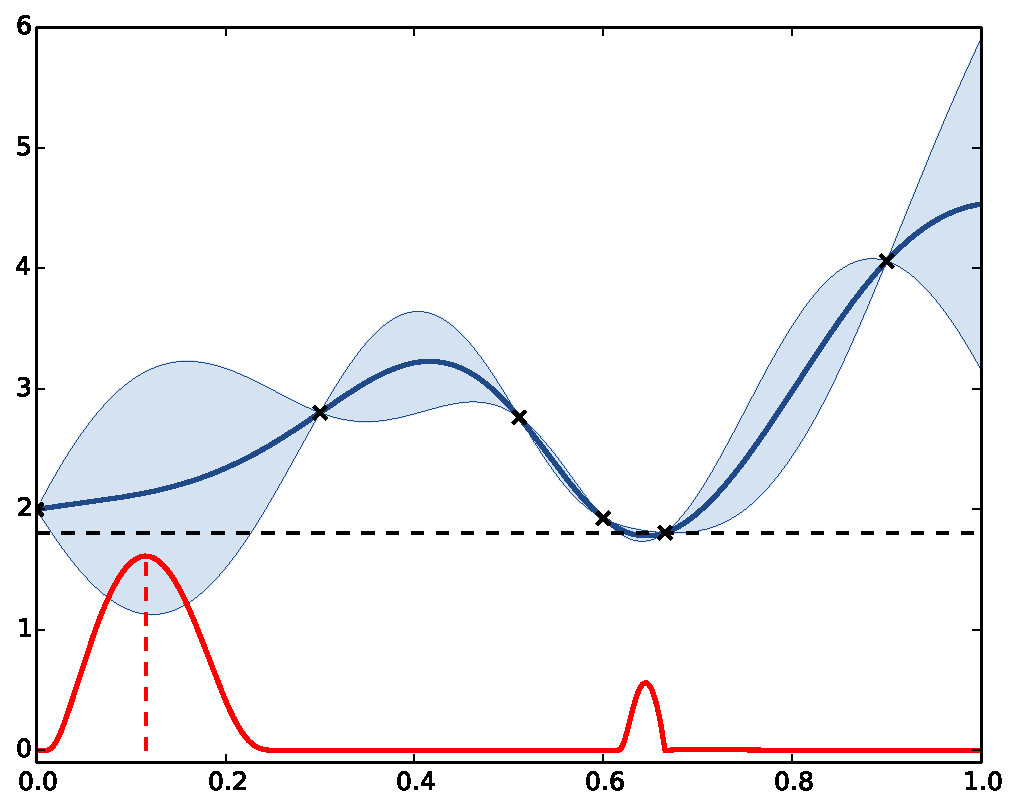
\includegraphics[height=5cm]{figures/python/ego_EI2}
\end{center}
\end{frame}

%%%%%%%%%%%%%%%%%%%%%%%%%%%%%%%%%%%%%%%%%%%%%%%%%%%%%%
\begin{frame}[noframenumbering]{Expected Improvement}
Let's see how it works... iteration 3
\begin{center}
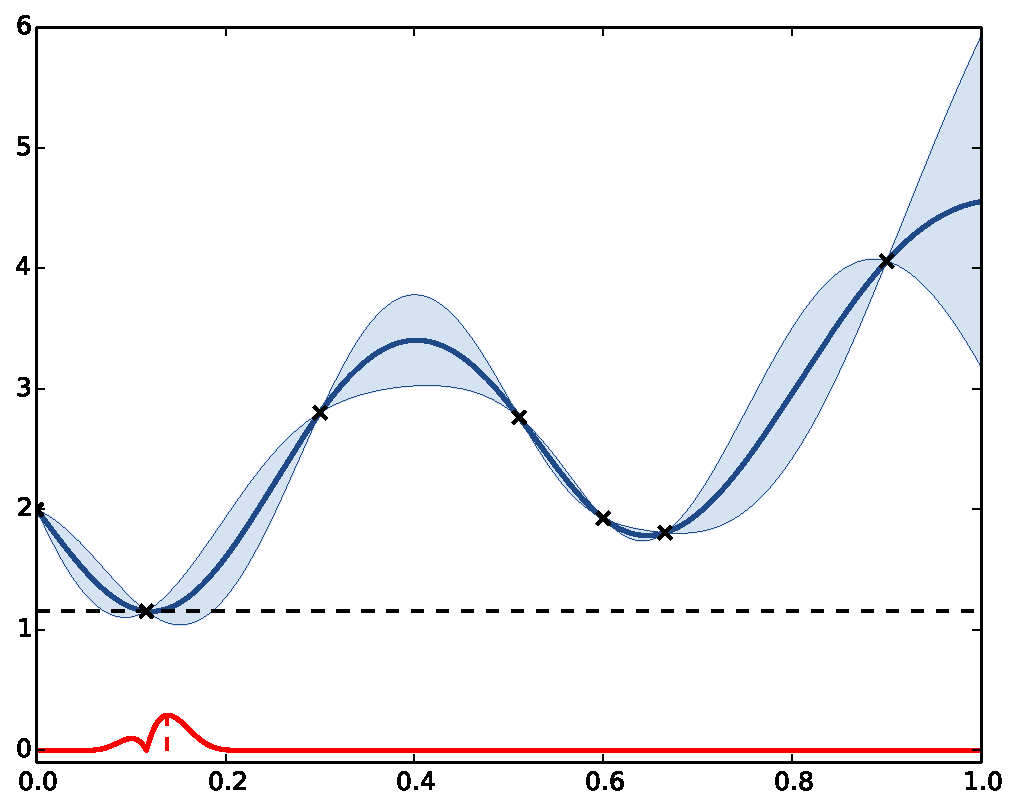
\includegraphics[height=5cm]{figures/python/ego_EI3}
\end{center}
\end{frame}

%%%%%%%%%%%%%%%%%%%%%%%%%%%%%%%%%%%%%%%%%%%%%%%%%%%%%%
\begin{frame}[noframenumbering]{Expected Improvement}
Let's see how it works... iteration 4
\begin{center}
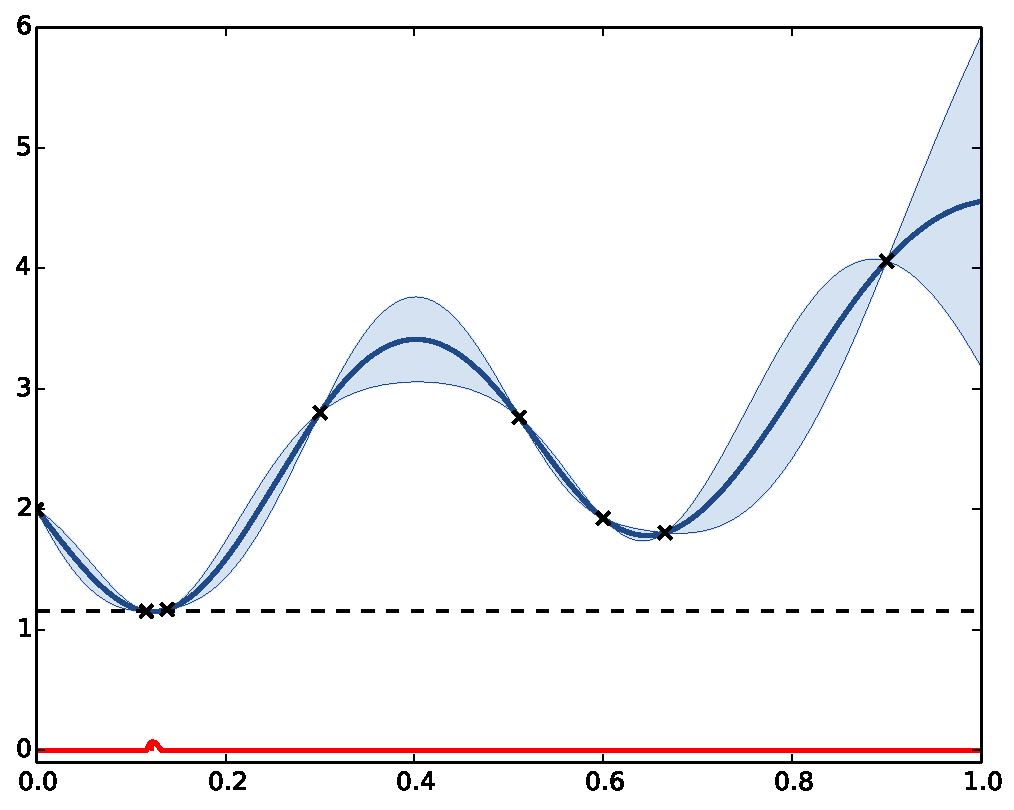
\includegraphics[height=5cm]{figures/python/ego_EI4}
\end{center}
\end{frame}

%%%%%%%%%%%%%%%%%%%%%%%%%%%%%%%%%%%%%%%%%%%%%%%%%%%%%%
\begin{frame}[noframenumbering]{Expected Improvement}
Let's see how it works... iteration 5
\begin{center}
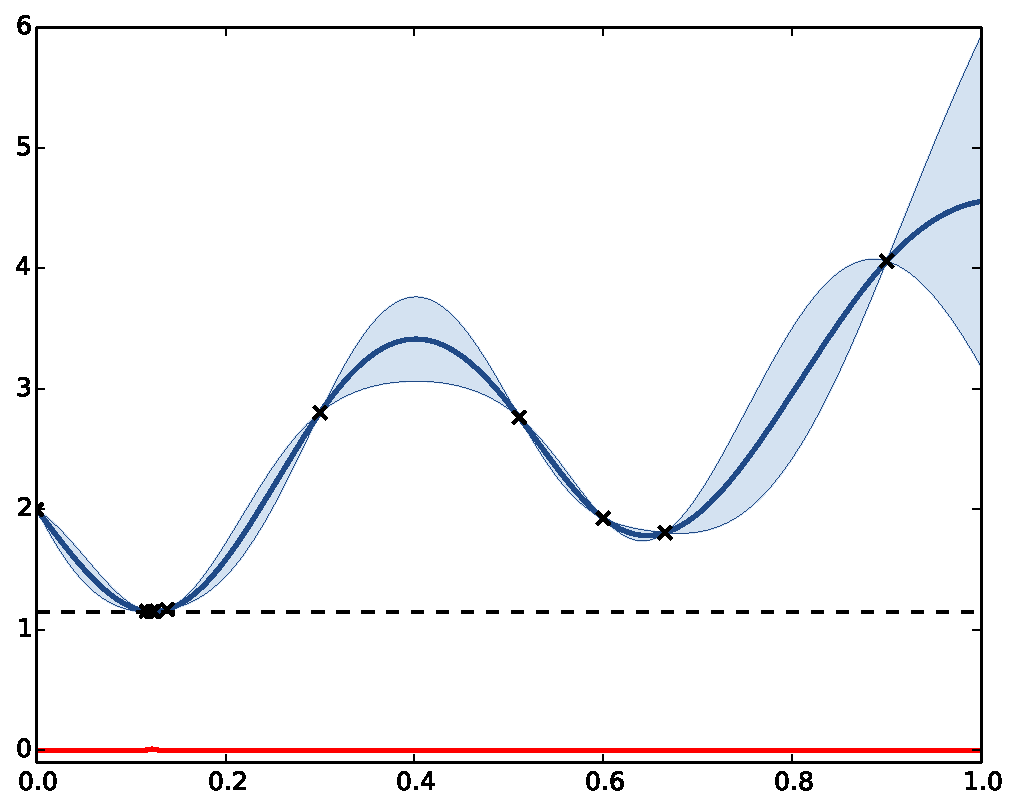
\includegraphics[height=5cm]{figures/python/ego_EI9}
\end{center}
\end{frame}

%%%%%%%%%%%%%%%%%%%%%%%%%%%%%%%%%%%%%%%%%%%%%%%%%%%%%%
\begin{frame}{}

\begin{exampleblock}{Illustration for $d=6$ (Hartman)}
	Illustration in higher dimension
\begin{center}
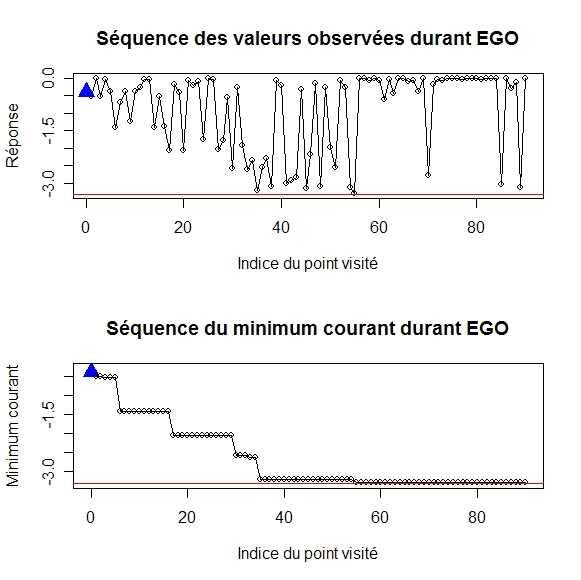
\includegraphics[height=5.5cm]{figures/egoHartman} 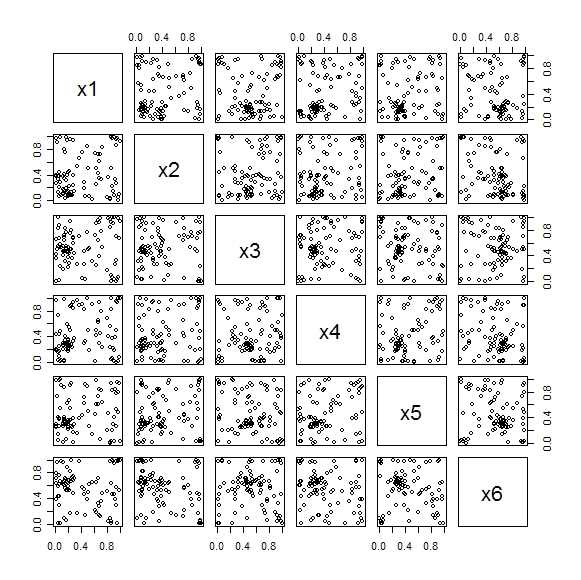
\includegraphics[height=5.5cm]{figures/egoHartman2}
\end{center}
\small Source: DiceOptim, D. Ginsbourger, 2009.
\end{exampleblock}
\end{frame}

%%%%%%%%%%%%%%%%%%%%%%%%%%%%%%%%%%%%%%%%%%%%%%%%%%%%%%
\begin{frame}{Expected Improvement}
This algorithm is called \textbf{Efficient Global Optimization} (EGO). It is famous since a paper of Jones et Al in 1998.\\
\vspace{5mm}
\begin{itemize}
	\item[+] EGO provides a good trade-off between exploitation and exploration.
	\item[+] It only requires a few function observations (10 in the example)
\end{itemize}
One issue is that we may have a model with observations very close one from each other\\
\begin{example}
From the previous 5 iterations, we obtain $1.44e39$ for the conditioning of the covariance matrix. Eigenvalues are
$$ (67.70,\  24.86,\  5.13,\  1.68,\  0.45,\  0.16,\  0.01,\  0.00,\  0.00,\ 0.00) $$
\end{example}
\end{frame}

%%%%%%%%%%%%%%%%%%%%%%%%%%%%%%%%%%%%%%%%%%%%%%%%%%%%%%
\begin{frame}{}
One way to improve the conditioning of the covariance matrix is to replace two values that are close-by by one function value and one derivative:
\begin{center}
  \begin{tabular}{ccc}
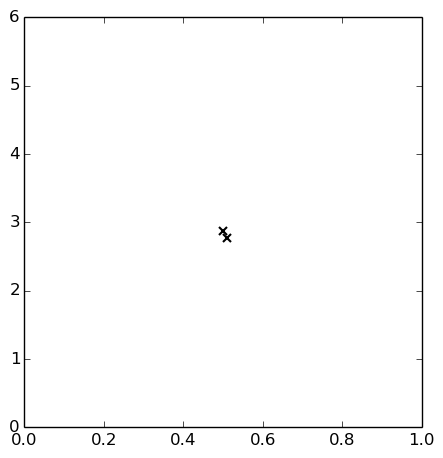
\includegraphics[height=4cm]{figures/python/osborn0} &

\includegraphics[height=4cm]{figures/Rightarrow} &
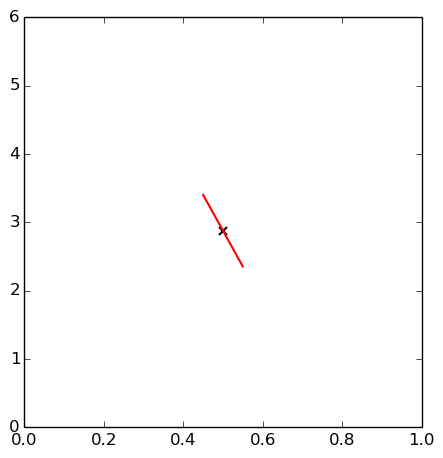
\includegraphics[height=4cm]{figures/python/osborn1} \\
Cond. = 3842 & & Cond. = 10
  \end{tabular}
\end{center}
This can be generalised to higher orders \alert{$\rightarrow$} Taylor expansion\\
\small see articles from M. Osborn
\end{frame}

%%%%%%%%%%%%%%%%%%%%%%%%%%%%%%%%%%%%%%%%%%%%%%%%%%%%%%
\begin{frame}{}
If we now the computational budget in advance, adding new points at the \textbf{best one step ahead location} is not optimal.\\
\vspace{5mm}
Some improvements have been made toward this
\begin{itemize}
	\item Batch EGO
	\item Parallelization of the algorithm
\end{itemize}
\vspace{5mm}
\small see works from D. Ginsbourger
\end{frame}

%%%%%%%%%%%%%%%%%%%%%%%%%%%%%%%%%%%%%%%%%%%%%%%%%%%%%%
%%%%%%%%%%%%%%%%%%%%%%%%%%%%%%%%%%%%%%%%%%%%%%%%%%%%%%
\section[Robust optim.]{Robust optimization}
\subsection{}

%%%%%%%%%%%%%%%%%%%%%%%%%%%%%%%%%%%%%%%%%%%%%%%%%%%%%%
\begin{frame}{}
Robust optimization may mean various things:
\begin{itemize}
	\item There is observation noise on the output
	\item Some input variables are uncertain
	\item Model is uncertain
\end{itemize}
\vspace{2mm}
\begin{example}
\begin{columns}[c]
\column{3cm}
	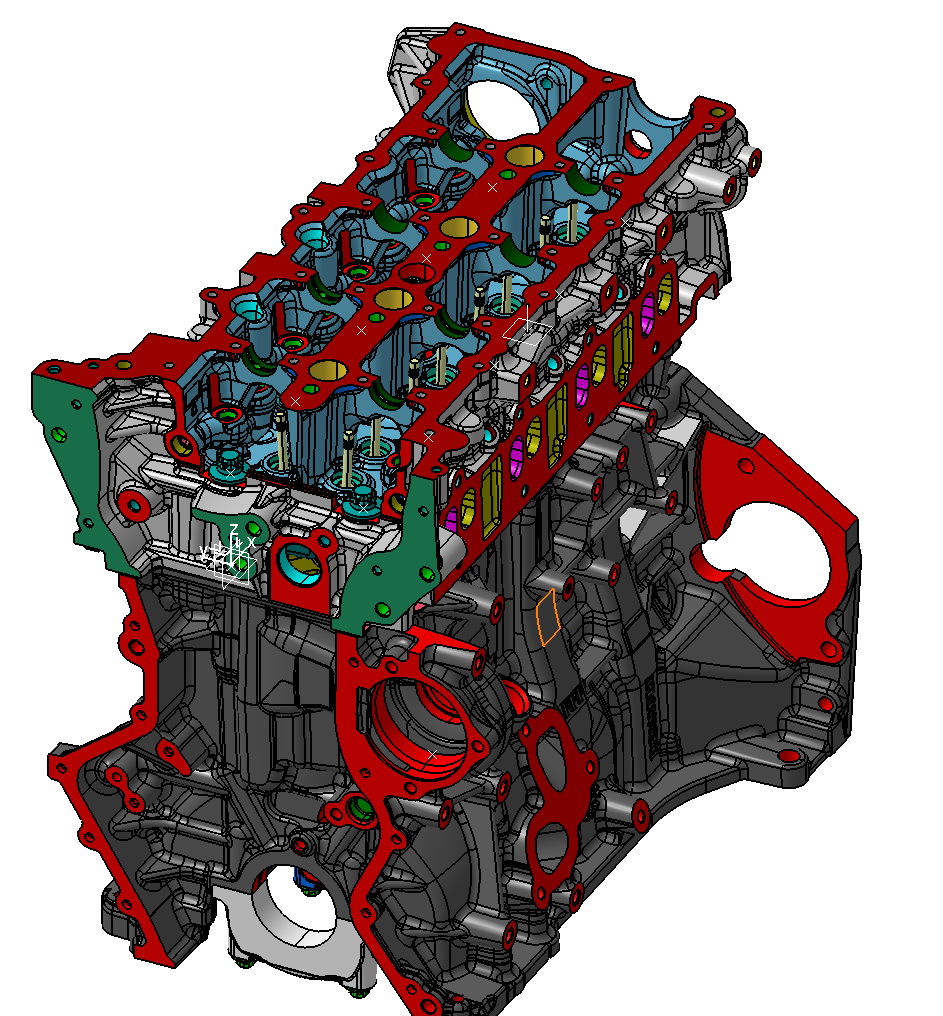
\includegraphics[height=4cm]{figures/RLRrobust}
\column{5cm}
	a +/- 1mm dispersion in the manufacturing of a car cylinder head  can degrade its performance (g CO2/km) by -20\% (worst case)\\
\end{columns}
\vspace{3mm}
	\small Source: Talk from R. Le Riche at the Porquerolles Summer School, 2014
\end{example}
\end{frame}

%%%%%%%%%%%%%%%%%%%%%%%%%%%%%%%%%%%%%%%%%%%%%%%%%%%%%%
\begin{frame}{}
% \begin{example}
% Here is a basic example:
% \begin{center}
% 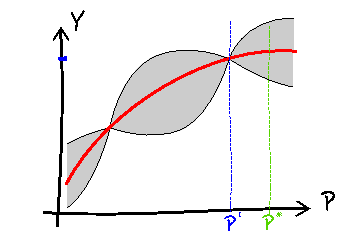
\includegraphics[height=5cm]{figures/optim_rob_a}\\
% Which input is the best?
% \end{center}
% \end{example}
% \end{frame}

% %%%%%%%%%%%%%%%%%%%%%%%%%%%%%%%%%%%%%%%%%%%%%%%%%%%%%%
% \begin{frame}[noframenumbering]{}
\begin{example}
Here is a basic example:
\begin{center}
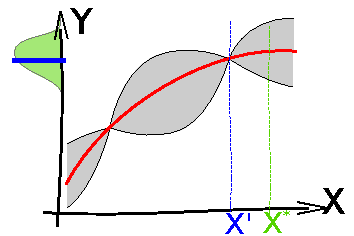
\includegraphics[height=5cm]{figures/optim_rob_b}\\
Which input is the best?
\end{center}
\end{example}
\end{frame}

%%%%%%%%%%%%%%%%%%%%%%%%%%%%%%%%%%%%%%%%%%%%%%%%%%%%%%
\begin{frame}[noframenumbering]{}
\begin{example}
A non Gaussian example
\begin{center}
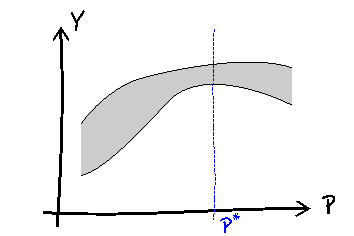
\includegraphics[height=5cm]{figures/optim_rob_c}\\
In some cases, we may want to optimize the worst case scenario. 
\end{center}
\end{example}
\end{frame}

%%%%%%%%%%%%%%%%%%%%%%%%%%%%%%%%%%%%%%%%%%%%%%%%%%%%%%
\begin{frame}{}
Can EGO be adapted when observations are noisy?\\
\vspace{5mm}
First of all, using the current best observation as a minimum does not make much sense...\\
\vspace{5mm}
Some solutions are
\begin{itemize}
	\item[S1] Build a new model that interpolates $m(X)$ at $X$. 
	\item[S2] Include observation noise and replace $\min(F)$ by $\min(m(X))$ in the EI expression
	\item[S3] Similar to 2 but consider an Expected Mean Improvement.
\end{itemize}
\end{frame}

%%%%%%%%%%%%%%%%%%%%%%%%%%%%%%%%%%%%%%%%%%%%%%%%%%%%%%
\begin{frame}{Solution 1}
iteration 0
\begin{center}
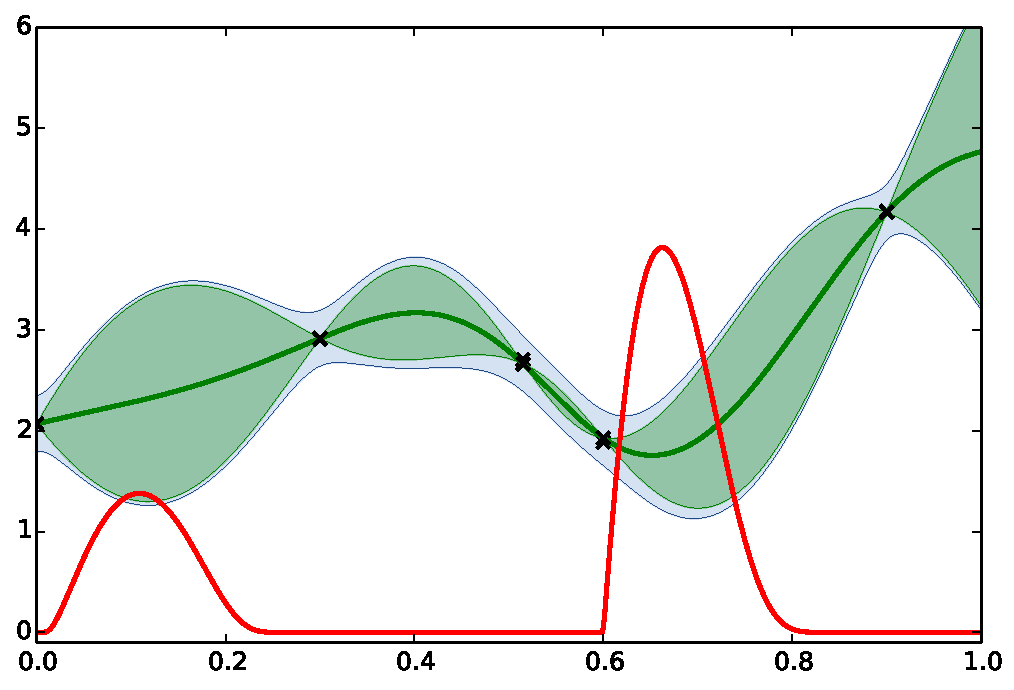
\includegraphics[height=5cm]{figures/python/ego_EI1n0}
\end{center}
\end{frame}

%%%%%%%%%%%%%%%%%%%%%%%%%%%%%%%%%%%%%%%%%%%%%%%%%%%%%%
\begin{frame}[noframenumbering]{Solution 1}
iteration 1
\begin{center}
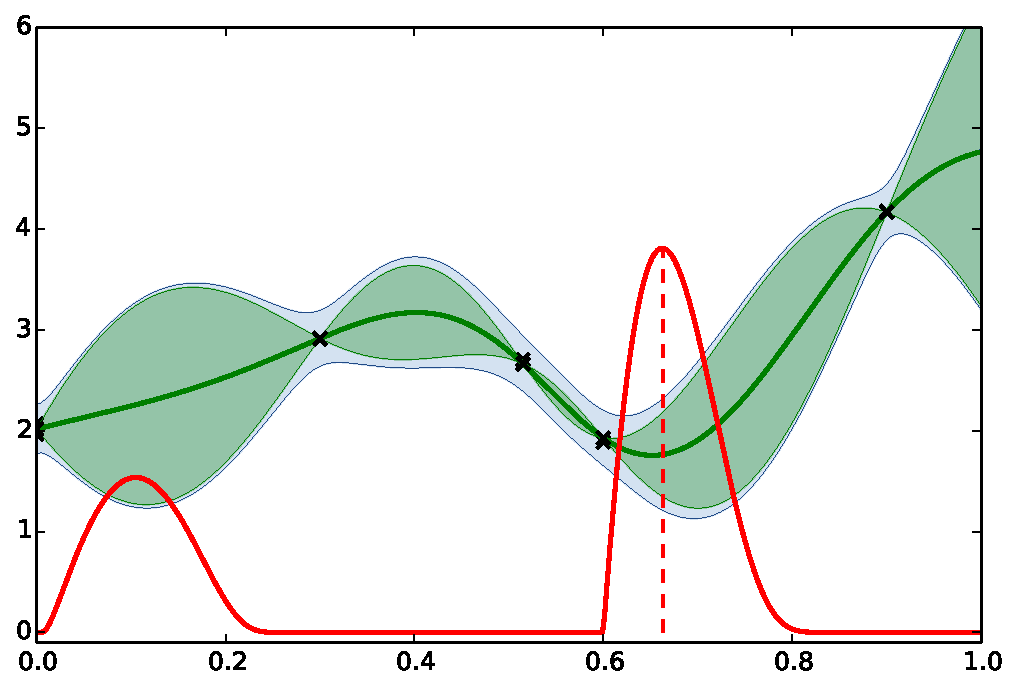
\includegraphics[height=5cm]{figures/python/ego_EI1n1}
\end{center}
\end{frame}

%%%%%%%%%%%%%%%%%%%%%%%%%%%%%%%%%%%%%%%%%%%%%%%%%%%%%%
\begin{frame}[noframenumbering]{Solution 1}
iteration 2
\begin{center}
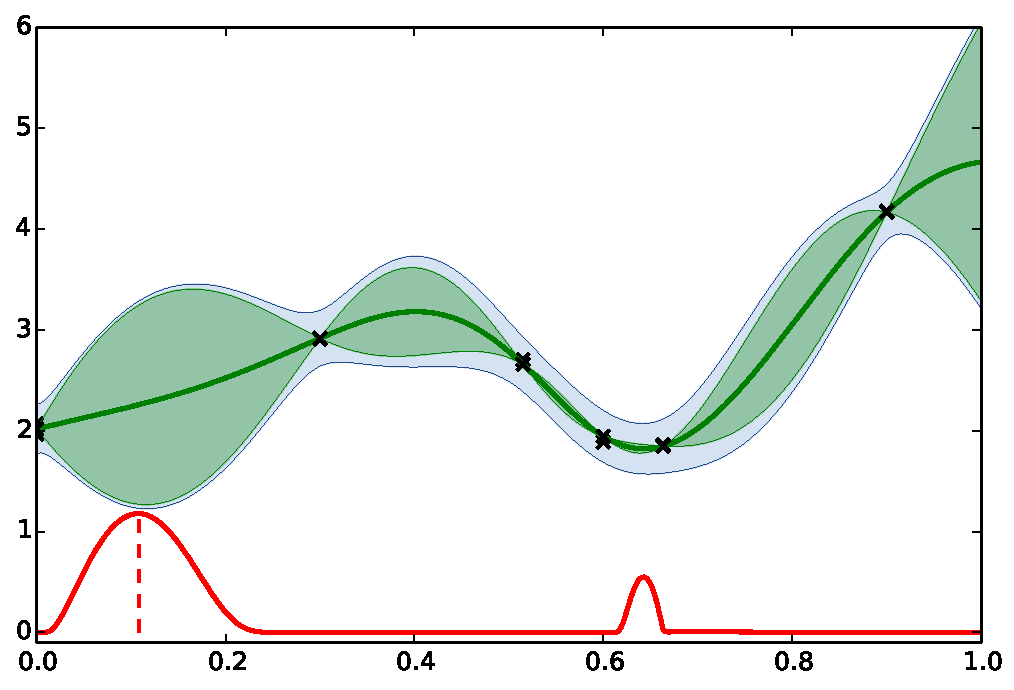
\includegraphics[height=5cm]{figures/python/ego_EI1n2}
\end{center}
\end{frame}

%%%%%%%%%%%%%%%%%%%%%%%%%%%%%%%%%%%%%%%%%%%%%%%%%%%%%%
\begin{frame}[noframenumbering]{Solution 1}
iteration 3
\begin{center}
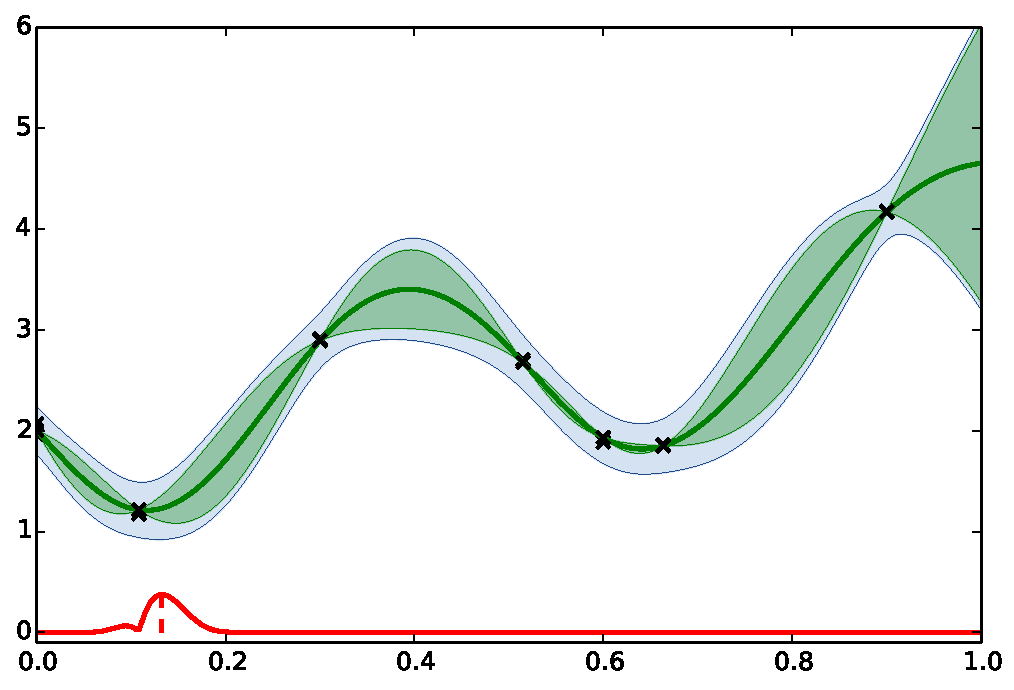
\includegraphics[height=5cm]{figures/python/ego_EI1n3}
\end{center}
\end{frame}

%%%%%%%%%%%%%%%%%%%%%%%%%%%%%%%%%%%%%%%%%%%%%%%%%%%%%%
\begin{frame}[noframenumbering]{Solution 1}
iteration 4
\begin{center}
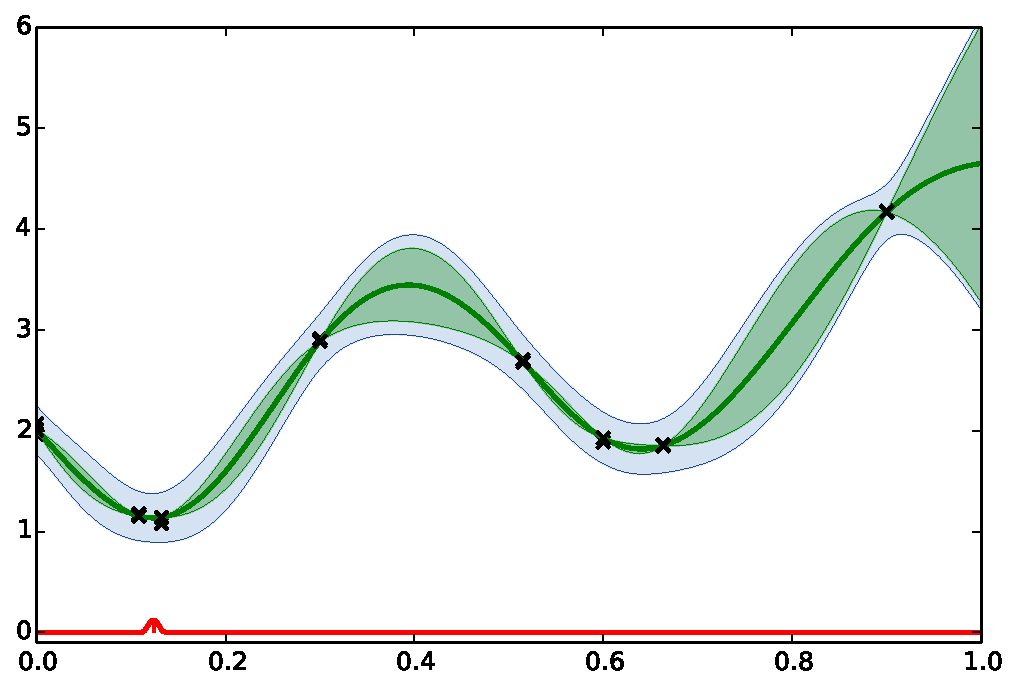
\includegraphics[height=5cm]{figures/python/ego_EI1n4}
\end{center}
\end{frame}

%%%%%%%%%%%%%%%%%%%%%%%%%%%%%%%%%%%%%%%%%%%%%%%%%%%%%%
%%%%%%%%%%%%%%%%%%%%%%%%%%%%%%%%%%%%%%%%%%%%%%%%%%%%%%
\section[Related problems]{Related problems}
\subsection{}

%%%%%%%%%%%%%%%%%%%%%%%%%%%%%%%%%%%%%%%%%%%%%%%%%%%%%%
\begin{frame}{}
Some related optimization problems are:
\begin{itemize}
	\item calibration problems
	\item probability computations
\end{itemize}
\vspace{8mm}
Some algorithms with an EGO spirit can be applied:
\begin{itemize}
 	\item SUR methods
 \end{itemize} 
\end{frame}

%%%%%%%%%%%%%%%%%%%%%%%%%%%%%%%%%%%%%%%%%%%%%%%%%%%%%%
\begin{frame}{}
We want to find the input(s) such that f(x) = 3.2
\begin{center}
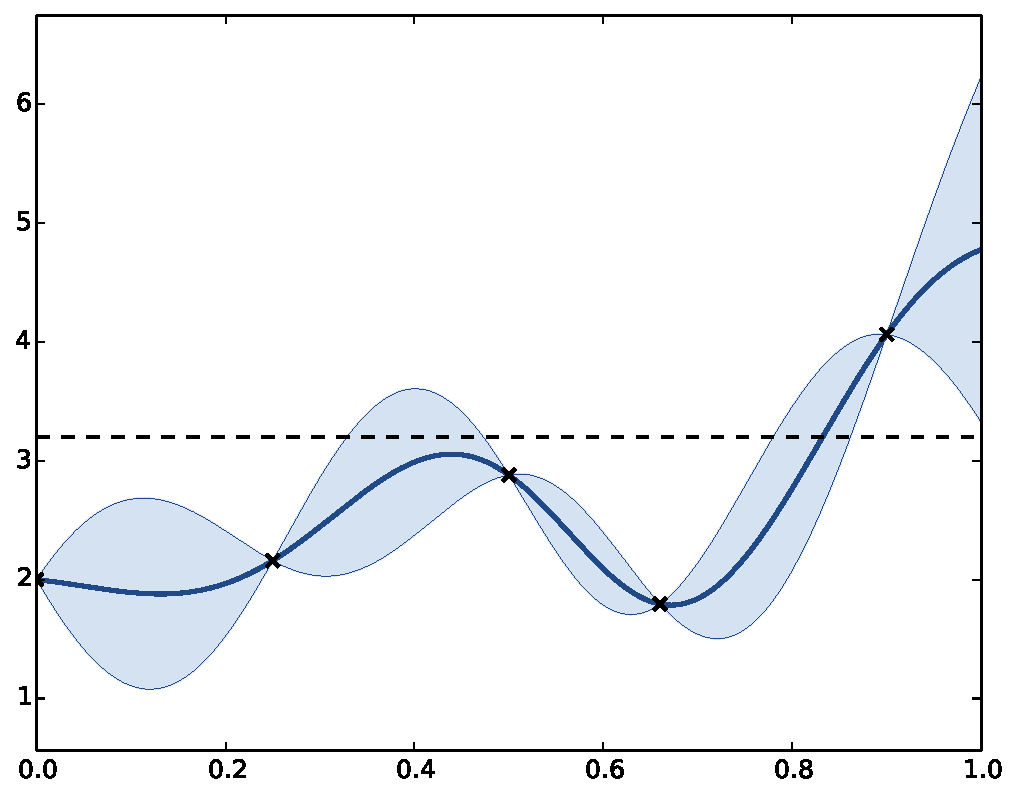
\includegraphics[height=5cm]{figures/python/inv}
\end{center}
\end{frame}

%%%%%%%%%%%%%%%%%%%%%%%%%%%%%%%%%%%%%%%%%%%%%%%%%%%%%%
\begin{frame}[noframenumbering]{}
iteration 0: 
\begin{center}
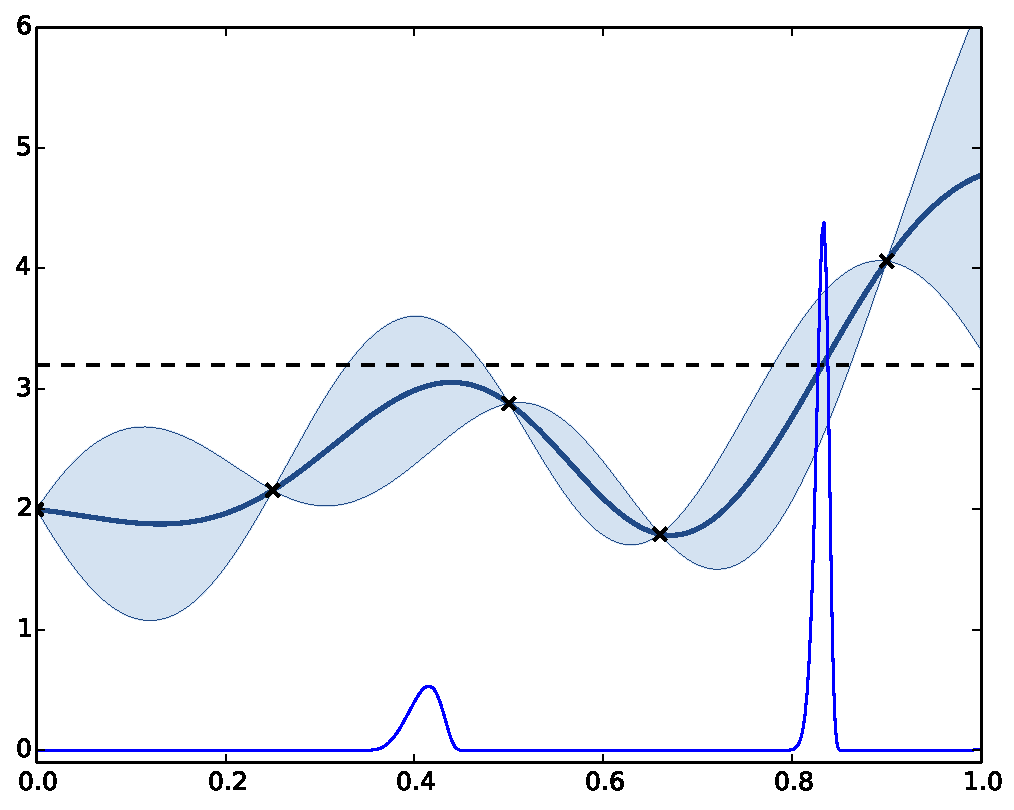
\includegraphics[height=5cm]{figures/python/invproba}
\end{center}
\end{frame}

%%%%%%%%%%%%%%%%%%%%%%%%%%%%%%%%%%%%%%%%%%%%%%%%%%%%%%
\begin{frame}[noframenumbering]{}
iteration 1: 
\begin{center}
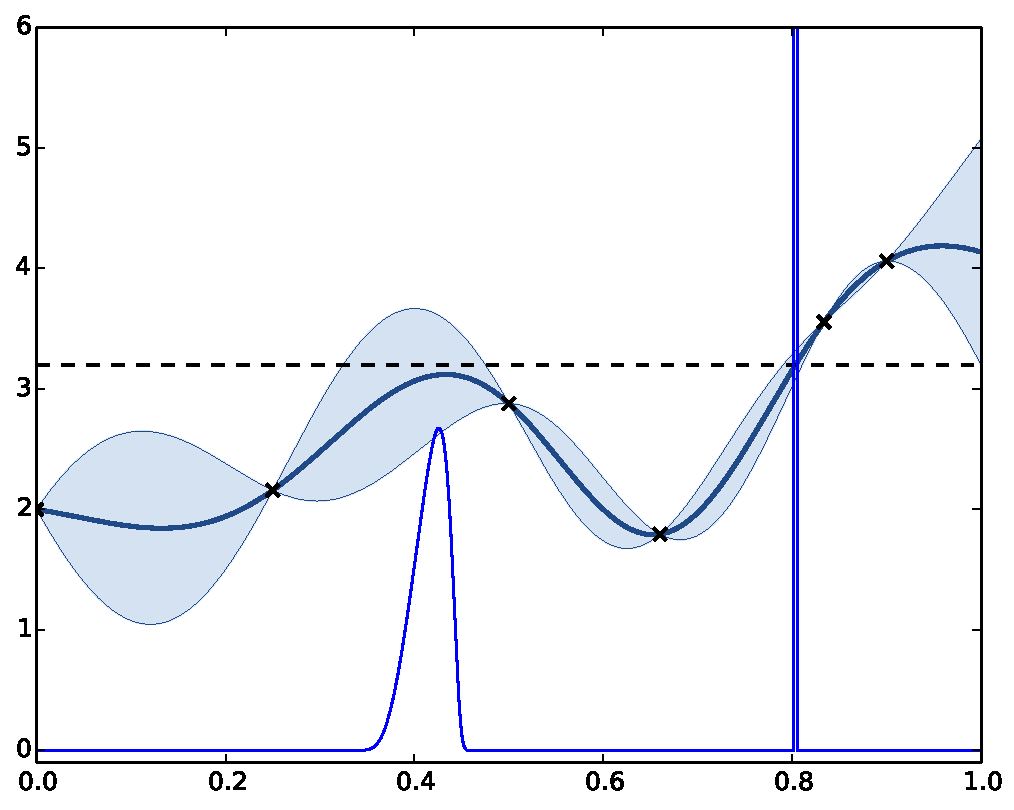
\includegraphics[height=5cm]{figures/python/invproba1}
\end{center}
\end{frame}

%%%%%%%%%%%%%%%%%%%%%%%%%%%%%%%%%%%%%%%%%%%%%%%%%%%%%%
\begin{frame}[noframenumbering]{}
iteration 2: 
\begin{center}
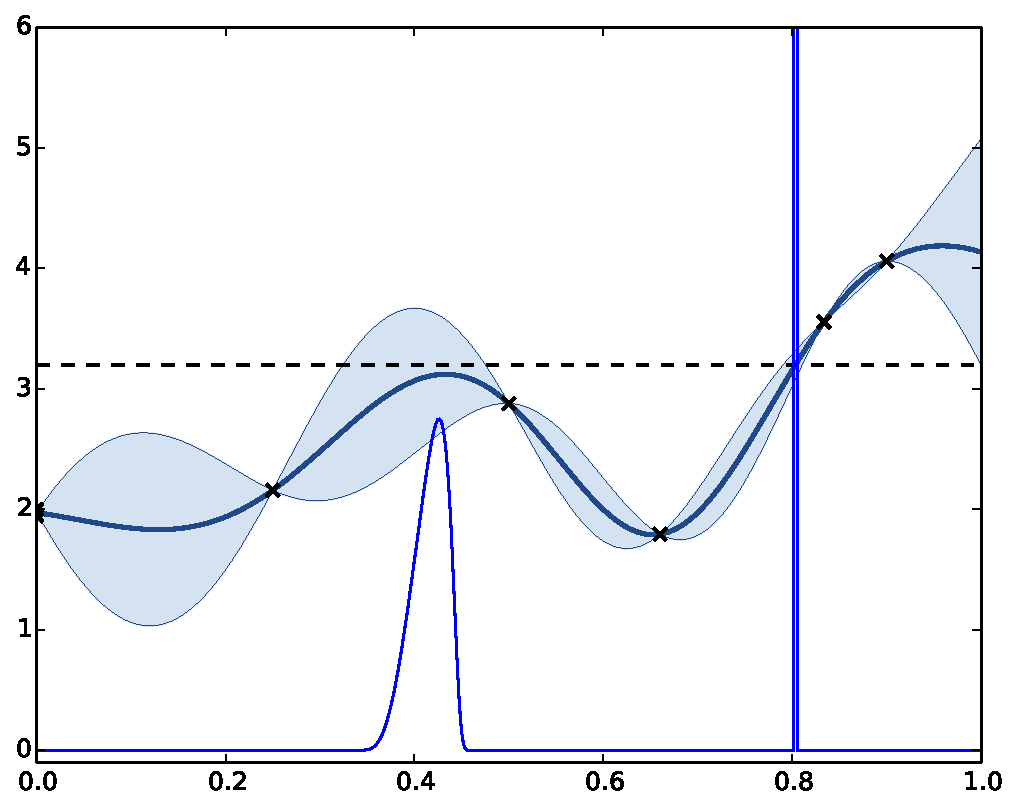
\includegraphics[height=5cm]{figures/python/invproba2}
\end{center}
\end{frame}

%%%%%%%%%%%%%%%%%%%%%%%%%%%%%%%%%%%%%%%%%%%%%%%%%%%%%%
\begin{frame}[noframenumbering]{}
iteration 3: 
\begin{center}
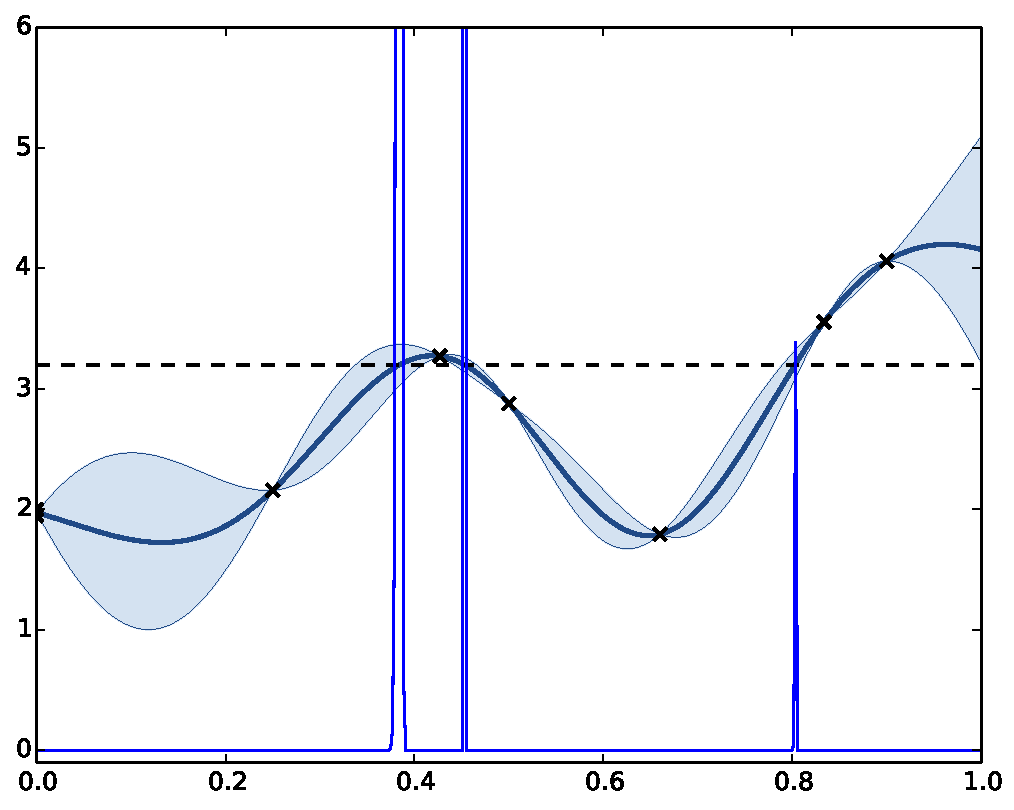
\includegraphics[height=5cm]{figures/python/invproba3}
\end{center}
\end{frame}

%%%%%%%%%%%%%%%%%%%%%%%%%%%%%%%%%%%%%%%%%%%%%%%%%%%%%%
%%%%%%%%%%%%%%%%%%%%%%%%%%%%%%%%%%%%%%%%%%%%%%%%%%%%%%
\section[Concl]{Conclusion}
\subsection{}

%%%%%%%%%%%%%%%%%%%%%%%%%%%%%%%%%%%%%%%%%%%%%%%%%%%%%%
\begin{frame}[noframenumbering]{}
Usual optimization methods such as 
\begin{itemize}
	\item gradient based methods
	\item evolutionary/genetic algorithms
\end{itemize}
are not relevant for costly to evaluate functions.\\
\vspace{5mm}
Once again, statistical models can be of great help...
\begin{itemize}
	\item few number of function evaluations
	\item good noise filtering
	\item trade-off exploitation/exploration available
\end{itemize}
\end{frame}

%%%%%%%%%%%%%%%%%%%%%%%%%%%%%%%%%%%%%%%%%%%%%%%%%%%%%%%%%%%%%%%%%%%%%%%%%%%%%%%
%%%%%%%%%%%%%%%%%%%%%%%%%%%%%%%%%%%%%%%%%%%%%%%%%%%%%%%%%%%%%%%%%%%%%%%%%%%%%%%
%%%%%%%%%%%%%%%%%%%%%%%%%%%%%%%%%%%%%%%%%%%%%%%%%%%%%%%%%%%%%%%%%%%%%%%%%%%%%%%
%%%%%%%%%%%%%%%%%%%%%%%%%%%%%%%%%%%%%%%%%%%%%%%%%%%%%%%%%%%%%%%%%%%%%%%%%%%%%%%
\end{document}


%%%%%%%%%%%%%%%%%%%%%%%%%%%%%%%%%%%%%%%%%%%%%%%%%%%%%%
%%%%%%%%%%%%%%%%%%%%%%%%%%%%%%%%%%%%%%%%%%%%%%%%%%%%%%
%%%%%%%%%%%%%%%%%%%%%%%%%%%%%%%%%%%%%%%%%%%%%%%%%%%%%%

\structure{}

\begin{center}
  \begin{tabular}{|c|cc|}

  \end{tabular}
\end{center}

###
%%%%%%%%%%%%%%%%%%%%%%%%%%%%%%%%%%%%%%%%%%%%%%%%%%%%%%
\begin{frame}{}

\end{frame}

###
\begin{block}{}

\end{block}

###
\begin{center}
\includegraphics[height=5cm]{figures/}
\end{center}

###
\begin{columns}[c]
\column{5cm}

\column{5cm}

\end{columns}
